
\section{Diskrete Modelle}

\begin{Definition}[Laplace Wahrscheinlichkeit]
Sei $\Omega = \{ \omega_1, \cdots , \omega_n\}$ eine endliche Menge. Für $A \subset \Omega$ definieren wir die Wahrscheinlichkeit durch
\begin{align*}
P(A) : = \frac{\#A}{ \# \Omega} \; . 
\end{align*} 
Die Elemente $ \omega_1, \cdots , \omega_n \in \Omega$ nennen wir Elementarereignisse und Teilmengen $A \subset \Omega$ Ereignisse. Die Abbildung
\begin{align*}
P : \mathcal{P} (\Omega) \to [0,1]  
\end{align*}  
nennen wir die Laplace-Verteilung bzw. Gleichverteilung auf $\Omega$.
\end{Definition}


\begin{Definition}[Permutationen und Kombinationen]

\begin{itemize}
\item $Perm_k^n(\Omega, m.W.) : = \{ \omega_1, \ldots, \omega_k \in \Omega^k \}$  Menge aller Permutationen mit Wiederholung.
\item $Perm_k^n(\Omega, o.W.) : = \{ \omega_1, \ldots, \omega_k \in \Omega^k  | \omega_i \neq \omega_j\}$  Menge aller Permutationen ohne Wiederholung.
\item $Kom_k^n(\Omega, m.W.) : = \{ \omega_{i_1}, \ldots, \omega_{i_k} \in \Omega^k  | 1  \leq i_1 \leq  \ldots  \leq i_k \}$  Menge aller Kombinationen  mit Wiederholung.
\item $Kom_k^n(\Omega, o.W.) : = \{ \omega_{i_1}, \ldots, \omega_{i_k} \in \Omega^k  | 1 \leq i_1  \leq \ldots \leq i_k ;  \omega_{i_i} \neq \omega_{i_j} \}$  Menge aller Kombinationen  ohne  Wiederholung.
\end{itemize}
\end{Definition}

\begin{Lemma}
\begin{itemize}
\item $\# Perm_k^n(\Omega, m.W.)  = n^k = \underbrace{n \cdot n \cdots n}_{\text{k-mal}}$
\item $\# Perm_k^n(\Omega, o.W.)  = n_k = n \cdot (n-1) \cdots  (n-(k-1)) = \frac{n!}{(n-k)!}$  
\item $\#Kom_k^n(\Omega, o.W.) = \binom{n}{k} = \frac{n!}{k! (n-k)!}$  
\item $\#Kom_k^n(\Omega, m.W.)  = \binom{n + k -1}{k}$  
\end{itemize}
\end{Lemma}
\begin{proof}
\end{proof}


\begin{Definition}{Diskrete Wahrscheinlichkeitsverteilung}
Es sei $\Omega$ eine (nicht leere) albzählbare Menge. Eine Abbildung 
$P :\mathcal{P}(\Omega) \to [0,1]$ heißt diskrete Wahrscheinlichkeitsverteilung (Wahrscheinlichkeismaß), falls gilt:
\begin{align*}
& P(\Omega) = 1\\
& P \Biggl( \bigcup_{n=1}^{\infty} A_n \biggr)= \sum_{n=1}^{\infty} P(A_n), \text{ mit } A_i \cap A_j = \emptyset \text{ für } i \neq j 
\end{align*}
\end{Definition}


\begin{Beispiel}{Beispiel: Laplace Wahrscheinlichkeit}
$\Omega$ endlich und $P(A) = \frac{\#A}{\#\Omega}$.
 \end{Beispiel}


\begin{Definition}{Bedingte  Wahrscheinlichkeit}
Für $A,B \subset \mathcal{P}(\Omega)$ und $P(B) > 0$ heißt
\begin{align*}
& P(A \; | \;  B) = \frac{P(A \cap B)}{P(B)} \\
\end{align*}
die bedingte Wahrscheinlichkeit (von $A$ unter $B$).
\end{Definition}


\begin{figure}[htp]
      \centering
    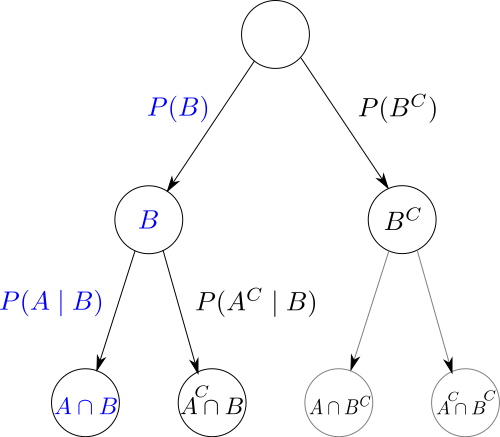
\includegraphics[width=0.5\textwidth]{images/Probability_tree}

      \caption{Quelle: Wikipedia}
\end{figure}



\begin{Satz}{Satz der totalen Wahrscheinlichkeit}
Für eine Zerlegung  $\Omega = \bigcup_{j=1}^{n} B_j, \text{ mit } B_i \cap B_k = \emptyset \text{ für } i \neq k $
\begin{align*}
& P(A ) = \sum_{j=1}^{n}  P(A \; | \;  B_j) \cdot P(B_j)
\end{align*}
\end{Satz}
\begin{proof}
$A = A \cap B \cup A \cap \bar{B}$ und  $A \cap B \cap A \cap \bar{B} = \emptyset$. 
\begin{align*}
& P(A) =  P(A \cap B) + P(A \cap \bar{B}) = P(B) \cdot P(A  \; | \; B) + P(\bar{B}) \cdot P(A  \; | \; \bar{B}) 
\end{align*}
\end{proof}

\begin{Satz}{Satz von Bayes}
Für $A,B \subset \mathcal{P}(\Omega)$ mit  $P(B) > 0$ gilt
\begin{align*}
& P(A \; | \;  B) = \frac{P(B \; | \; A) \cdot P(A)} {P(B)} \\
\end{align*}
\end{Satz}

\begin{proof}
\begin{align*}
& P(A \; | \;  B) =\frac{P(A \cap B)}{P(B)} = \frac{ \frac{P(A \cap B) \cdot P(A)}{P(A)}}{P(B)}  =  \frac{P(B \; | \; A) \cdot P(A)} {P(B)} 
\end{align*}
\end{proof}


\begin{Definition}{Stochastische Unabhängigkeit}
Zwei Ereignisse $A,B$ heißen stochastisch Unabhängig, falls
\begin{align*}
P(A \cap B) = P(A) \cdot P(B)
\end{align*}
gilt.  Somit ist auch $P(A | B) = P(A)$ und $P(B  | A) = P(B)$.
\end{Definition}


\subsection{Naiver Bayes'scher Spam Filter}
Gegeben ist eine E-Mail $E$.  Wir möchten anhand des Vorkommens bestimmter Wörter $A_1, \ldots A_n$ in der Mail entscheiden, ob es sich um eine erwünschte Mail $H$ oder eine unerwünschte Mail $S$ (Ham or Spam) handelt. 
(Typische Wörter wären zum Beispiel "reichwerden",  "onlinecasino" ...)
Aus einer Datenbank kann man das Vorkommen dieser Wörter in Spam und Ham Mails zählen und damit empirisch die Wahrscheinlichkeiten $P(A_i | S)$ und $P(A_i | H) $ des Vorkommens dieser Wörter in Spam und Ham Mails ermitteln.  Wir gehen davon aus, dass es sich bei der Mail  prinzipiell mit  Wahrscheinlichkeit $P(E= S) = P(E= H)= \frac{1}{2}$  um eine erwünschte  Mail $H$ oder eine unerwünschte Mail $S$  handeln kann. 




 Wir machen zudem die (naive) Annahme, dass das Vorkommen der Wörter  stochastisch unabhängig ist, also 
\begin{align*}
P(A_1 \cap \cdots \cap A_n | S) = P(A_1 | S) \cdots P(A_n | S) \\
P(A_1 \cap \cdots \cap A_n | H) = P(A_1 | H) \cdots P(A_n | H)
\end{align*}
gilt.


Mit der Formel von Bayes und der totalen Wahrscheinlichkeit  können wir somit berechnen
\begin{align*}
& P(E=S |  A_1 \cap \cdots \cap A_n) = \frac{P(A_1 \cap \cdots \cap A_n | S) \cdot P(S)}{P(A_1 \cap \cdots \cap A_n)} \\
&=  \frac{P(A_1 | S) \cdots P(A_n | S) \cdot P(S)}{P(A_1 \cap \cdots \cap A_n | H) + P(A_1 \cap \cdots \cap A_n | S)} \\
&=  \frac{P(A_1 | S) \cdots P(A_n | S) \cdot P(S)}{P(A_1 | H) \cdots P(A_n | H)  + P(A_1 | S) \cdots P(A_n | S) } \\
\end{align*}
Bemerkung: $P(E=H |  A_1 \cap \cdots \cap A_n) = 1- P(E=S |  A_1 \cap \cdots \cap A_n) $


\section{Zufalssvariablen}

\begin{Definition}
Ein Messraum ist ein Paar $(\Omega, \mathcal{A})$ bestehend aus einer Menge $\Omega$ und einer Sigma-Algebra $\mathcal{A} \subset \mathcal{P}(\Omega)$.
\end{Definition}



\begin{Definition}
Sei $(\Omega, \mathcal{A}, P)$ ein Wahrscheinlichkeitsraum und $(\Omega', \mathcal{A}')$ ein Messraum. Eine Zufallsvariable ist eine Abbildung
$$X : \Omega \to \Omega'$$ 
so dass für alle Ereignisse $A' \in  \mathcal{A}'$
$$ X^{-1} (A') \in \mathcal{A}$$
 ein Ereignis in $\mathcal{A}$ ist. Urbilder von Ereignissen sind also Ereignisse.
\end{Definition}

\begin{Definition}
Sei $(\Omega, \mathcal{A}, P)$ ein Wahrscheinlichkeitsraum, $(\Omega', \mathcal{A}')$ ein Messraum und  $X : \Omega \to \Omega'$  Eine Zufallsvariable. 
Durch $P_X (A') := P(X^{-1} (A))$ für $A' \in \mathcal{A}'$ wird ein Wahrscheinlichkeitsmaß auf  $(\Omega', \mathcal{A}')$ definiert. Es wird Bildmaß genannt.
\end{Definition}



\subsection{Integration bezüglich eines Wahrscheinlichkeitsmaßes}
in diesem Abschnitt ist  $(\Omega, \mathcal{A},P)$ ein fest gewählter Wahrscheinlichkeitsraum.

\begin{Definition}
Für eine Teilmenge $A \in \mathcal{A}$ heißt
$$ 1_A (x): = \begin{cases} 1 \text{  falls }   x \in A  \\  0  \text{  sonst}  \end{cases}$$
Indikatorfunktion.
\end{Definition}

\begin{Definition}
Eine Funktion 
$$ \varphi(x) := \sum_{k=1}^m c_k 1_{A_k}$$ mit $c_k \in \mathbb{R}$ und $A_k \in \mathcal{A}$ mit $A_l \cap A_h = \emptyset$ für $i \neq j$
heißt Treppenfunktion.
\end{Definition}





\begin{Definition}
Eine Hüllreihe zu einer Funktion $f :\Omega \to \mathbb{R}$ ist eine Reihe $\phi(x):= \sum_{k=1}^{\infty} c_k  1_{A_k} (x)$ mit den folgenden Eigenschaften:
\begin{itemize}
\item $c_k \in \mathbb{R}$ sind positive reelle Zahlen $c_k >0$.
\item $A_k \subset \mathcal{A}$.
\item Für alle $x \in \Omega$ gilt $|f(x) | \leq \phi(x)$.
\end{itemize}
\end{Definition}

 
\begin{Definition}
Für eine Treppenfunktion $ \varphi(x) := \sum_{k=1}^m c_k 1_{A_k}$ definieren wir das Integral durch
$$\int_{\mathbb{R}^n} \varphi dP := \sum_{k =1}^m  c_k P(A_k) \; . $$
\end{Definition}


\begin{Definition}
Der Innhalt einer Hüllreihe $\phi(x):= \sum_{k=1}^{\infty} c_k  1_{A_k} (x)$ ist definiert durch 
$$I_P (\phi) := \sum_{k=1}^{\infty} c_k \;  P(A_k) \; .$$
\end{Definition}


\begin{Definition}
Die $L_{P^1}$-Halbnorm einer Funktion $f : \Omega\to \mathbb{R}$ is definiert durch das Infimum der Inhalte der Hüllreihen zu $f$
$$ || f ||_{P^1} : = \inf  \biggl \{   I(\phi) \; | \; \phi  \text{ ist Hüllreihe zu  }  f \biggr \} \; .$$
\end{Definition}



\begin{Definition}
Eine Funktion $f : \Omega \to \mathbb{R}$ heißt integrierbar, falls eine Folge von Treppenfunktionen  $\varphi_k$ existiert mit
$$ || f -  \varphi_k ||_1 \to 0 \text{ für } k \to \infty \;. $$
In diesem Fall heißt
$$ \int_{\mathbb{R}^n} f(x) dP := \lim_{k \to \infty}  \int_{\mathbb{R}^n}  \varphi_k d dP$$
das Integral von $f$ über $\mathbb{R}^n$.
\end{Definition}


\subsection{Reelle Zufalssvariablen}

\begin{Definition}
Eine Menge $U \subset  \mathbb{R}^n$ heißt offen, falls für jeden Punkt $x \in U$ ein Radius $\epsilon > 0$ existiert, so dass der Ball $B_\epsilon (x)$ in $U$ enthalten ist, also 
$B_\epsilon (x) \subset U$ gilt.
\end{Definition}

\begin{figure}[htp]
      \centering
    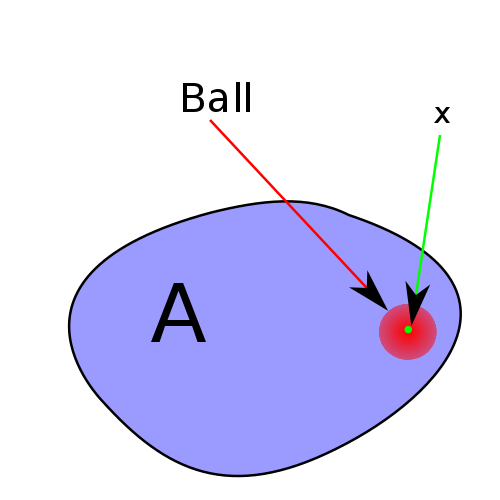
\includegraphics[width=0.45\textwidth]{images/openset}
      \caption{Quelle: Wikipedia}
\end{figure}


\begin{Definition}
Die Borel'sche   $\sigma$-Algebra $\mathcal{B}(\mathbb{R}^n$über $\mathbb{R}^n$ ist die kleinste  $\sigma$-Algebra, die alle offenen Mengen $\mathcal{U}$ enthält, also 
\begin{align*}
A_\sigma (\mathcal{U}) := \bigcap \{  \mathcal{A} \subset \mathcal{P}(\mathbb{R}^n);  \;   \mathcal{U}  \subset  \mathcal{A},  \;  \mathcal{A} \text{ ist $\sigma$-Algebra} \}
\end{align*}
\end{Definition}

\begin{Satz}
Die Borel'sche   $\sigma$-Algebra existiert, da die Potenzmenge eine   $\sigma$-Algebra ist.
\end{Satz}

\begin{Satz}
Die Borel'sche   $\sigma$-Algebra ist in der $\sigma$-Algebra der Lebesgue messbaren Mengen enthalten.
\end{Satz}

\begin{Definition}
Unter einer reellen Zufallsvariable verstehen wir eine Zufallsvariable $X : \Omega \to \mathbb{R}$, wobei $(\Omega, \mathcal{A}, P)$ ein Wahrscheinlichkeitsraum ist und $(\mathbb{R}, \mathcal{B}(\mathbb{R}^n)$ die reellen Zahlen zusammen mit der Borell'schen Sigma-Algebra ist.
\end{Definition}


\begin{Satz}
Eine reelle Zufallsvariable ist integrierbar.
\end{Satz}


\begin{Definition}
Für eine reelle Zufallsvariable ist der Erwartungswert definiert durch
$$ \mathbb{E} (X) := \int_{\Omega} X dP \; .$$
\end{Definition}

\begin{Satz}
Ist $(\Omega, \mathcal{A}, P)$ ein diskreter Wahrscheinlichkeitsraum, so ist
$$ \mathbb{E} (X) := \sum_{\omega \in \Omega}  \omega \cdot P(\omega)$$
\end{Satz}



